\documentclass{report}

\usepackage{../../../../../../LaTeX/marzstyle}

\runningheads{Computervision}{Assignment 02$_2$ - Report}

\setcounter{chapter}{2}


\begin{document}
	\section{Task}
	\startsection
		The task is to recreate a 3Dobject from 2 images which were taken from two different points in the world. Because there were some outliers given in the dataset, these must first be determined and extracted from the data set with the \textsc{Ransac} method. In the end the errors are computed by comparing the result with the optimal result.
	\closesection
	
	\section{Solution}
	\startsection
		In the \textsc{Ransac} method, first 8 random points of the dataset are selected and the fundamental matrix is calculated. This fundamental matrix is then applied on each point of one of the dataset and when multiplying this with the corresponding point from the other dataset and squaring the result, we will get the squared error, which means how much the $F*x_1$ does differ from $x_2$. Then we will compute how many of these squared errors are below the threshold and if this count is largest we have the best approximated fundamental matrix. With the most inliers subset again the fundamental matrix is computed and the check is done again in order to find the final inliers of \fancytextletter{F}. This will terminate if all of the used points to calculate \fancytextletter{F} are also inliers. \\
		With this \fancytextletter{F} the essential matrix \fancytextletter{E} is calculated. In order to extract the rotation and translation of this \fancytextletter{E} it must first be decomposed. This is done by applying the SVD decomposition and if det(U) < 0, U = -U and the same goes for V. Then both possible rotation matrices and the two possible translation vector are computed as follows:
		\begin{align*}
			R1 \ &= \  U * W.T * V \\
			R1 \ &= \  U * W * V \\
			& \textit{whereas } W \textit{ is} \begin{bmatrix} 0 & -1 & 0 \\ 1 & 0 & 0 \\ 0 & 0 & 1\end{bmatrix} \\
			t1 \ &= \ \textit{third column of U} \\
			t2 \ &= \ -t1
		\end{align*}
		In order to compute the error to the optimal result, first the optimal result must be calculated (I first calculated the transformation matrix from the right to the left camera, but because the result of Pr is the inverted result of that, which is also equal to the transformation matrix from left to right, I just inverted the result). First the Transformation matrix from the Right Camera to the World is computed which will look as the following:
		\[
			HT\_r\_to\_w \ = \  
			\begin{bmatrix}
				\ & \ & \ & \ \\
				\ & Rr & \ & tr \\
				\ & \ & \ & \ \\
				0 & 0 & 0 & 1
			\end{bmatrix}
		\]
		Keep in mind that in the translation vector the x-coordinate is the negative. \\
		Because we want to calculate the Right to Left Camera Transformation matrix, next the World to the Left Camera space transformation matrix is computed, which looks as the following : 
		\[
			HT\_w\_to\_l \ = \  
			\begin{bmatrix}
				\ & \ & \ & \ \\
				\ & Rl.T & \ & -Rl.T * tl \\
				\ & \ & \ & \ \\
				0 & 0 & 0 & 1
			\end{bmatrix}
		\]
		With this the Right to Left Camera Transformation matrix can be calculated:
		\[
			HT\_r\_to\_l \ = \ HT\_w\_to\_l * HT\_r\_to\_w
		\]
		By inverting this matrix as follows:
		\[
			inv(HT\_r\_to\_l) \ = \ 
			\begin{bmatrix}
				\ & \ & \ & \ \\
				\ & HT\_r\_to\_l[:3,:3].T & \ & -HT\_r\_to\_l[:3,:3] * HT\_r\_to\_l[:3,3] \\
				\ & \ & \ & \ \\
				0 & 0 & 0 & 1
			\end{bmatrix}
			\ = \ HT\_l\_to\_r
		\]
		, we can compare this "perfect" solution with the approximated solution $Pr$. In order to do that we need to normalize the translation vector of the result, because in the approximated solution the translation vector is also normalized. By extracting the rotation matrix and using the euler angles of it and translation vector we can calculate the L1-error.
	\closesection
	
	\section{Results}
	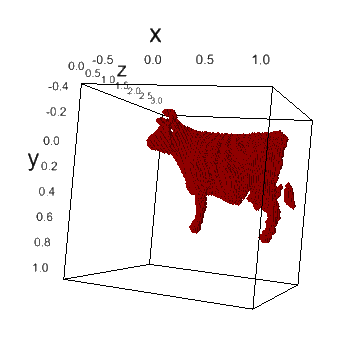
\includegraphics[scale=1]{3d_Result.png} \\
	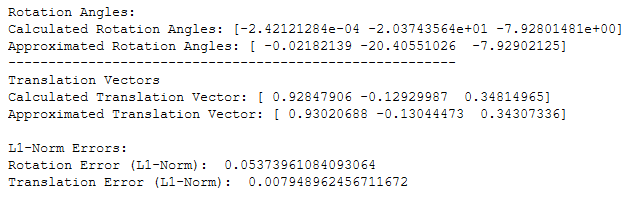
\includegraphics[scale=1]{Numeral_Results.png}
	\startsection
		As one can see the results are really good and the 3D object recreation works as intended. The highest error is with the x-Rotation, but because it is really near to 0 it does not matter as much and the result is still good
	\closesection
\end{document}